\newpage
\chapter{Simulation}

\section{Le simulateur : Omnet++}
OMNeT ++ est une bibliothèque et une structure de simulation C ++ extensible, modulaire et basée sur des composants, principalement utilisé pour la construction de simulateurs de réseau. Le terme "réseau" est entendu dans un sens plus large qui inclut les réseaux de communication câblés et sans fil, les réseaux sur puce, les réseaux de mise en file d'attente, et ainsi de suite. Les fonctionnalités spécifiques au domaine telles que la prise en charge de réseaux de capteurs, de réseaux ad-hoc sans fil, de protocoles Internet, de modélisation de performances, de réseaux photoniques, etc., sont fournies par des frameworks de modèles, développés en tant que projets indépendants. OMNeT ++ offre un IDE basé sur Eclipse, un environnement d'exécution graphique et une foule d'autres outils. Il existe des extensions pour la simulation en temps réel, l'émulation de réseau, l'intégration de base de données, l'intégration SystemC et plusieurs autres fonctions.
Même si OMNeT ++ n'est pas un simulateur de réseau en soi, il a acquis une grande popularité en tant que plate-forme de simulation de réseau dans la communauté scientifique ainsi que dans les milieux industriels, et a constitué une importante communauté d'utilisateurs.
Afin de réaliser un ensemble de test/simulation nous avons utilisé Omnet pour ce projet.

Le code des fichiers $C^{++}$ est mis à disposition en Annexes.
\section{Génération des graphes}
Nous avons choisi d'utiliser iGraph, afin de generer des graphes aléatoires.
iGraph est une collection de bibliothèque pour créer et manipuler des graphiques et analyser des réseaux. Il est écrit en C et existe également en tant que paquets Python et R. Il existe de plus une interface pour Mathematica. Le logiciel est largement utilisé dans la recherche universitaire en sciences de réseau et dans des domaines connexes.
iGraph a été développé par Gábor Csárdi et Tamás Nepusz. Le code source des paquets iGraph a été écrit en C. iGraph est disponible gratuitement sous GNU General Public License Version 2.

La génération se fait en plusieurs étapes : 
\begin{enumerate}
\item Récupération des arguments : Nombres de  \textit{LoRaWAN} Gateway, \textit{LoRa} Gateway et de Isolated node.	
\item Création du graphe et ajout du nombre de sommets dont on a besoin.
\item On connecte les  \textit{LoRaWAN} à une  \textit{LoRaWAN} gateway, par définitions ils sont enregistré à au moins une gateway  \textit{LoRaWAN}.
\item On connecte des Isolated Node de manière aléatoire à une LoRa Gateway (au moins une)
\item Ensuite on applique un deuxième tour d'association de noeud à des gateway 	basé sur une méthode  Erdös Renyi : On définit la probabilité d'existence entre deux nœuds, pour chaque couple de nœud, on tire au sort un nombre, si le nombre est inférieur on met le lien.
\item On écrit le fichier .ned qui décrit la configuration du graphe crée. 

\begin{minted}[
frame=lines,
framesep=2mm,
baselinestretch=1.2,
bgcolor=LightGray,
fontsize=\footnotesize,
linenos
]{python}
fic.write("\t\t\t" + ""+nomSommet0+"["+str(num_sommet0)+"].channelsO++" + " --> "
+"{delay="+str(delay1)+"ms;}" + " --> " +
""+nomSommet1+"["+str(num_sommet1)+"].channelsI++" + ";\n")
fic.write("\t\t\t" + ""+nomSommet0+"["+str(num_sommet0)+"].channelsI++" + " <-- "
 +"{delay="+str(delay2)+"ms;}" + " <-- " +
   ""+nomSommet1+"["+str(num_sommet1)+"].channelsO++" + ";\n")
\end{minted}

\end{enumerate}
Par exemple voici le résultat graphique réalisé avec GraphViz :

\begin{figure}[!ht]
\centering
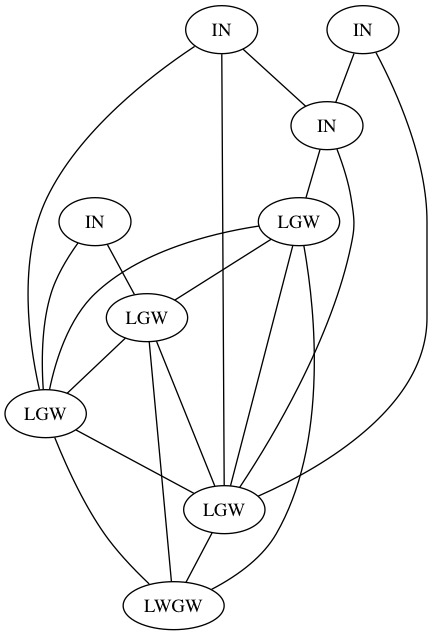
\includegraphics[scale=0.45]{LoRaGraph.jpg} 
\caption{Exemple de Graphe de sortie du script }
\end{figure}
Le code de génération de graphe aléatoire est mis à disposition dans son intégralité en Annexes.
\section{Représentation des échanges radio}
Dans cette version purement algorithmique sur Omnet++, la radio est definit par sa porté qui est donc la possibilité de communiqué avec un device. Si une arrête existe alors une communication est possible. Afin d'être plus réaliste, les arrêtes on pour attribut une latence, qui est générer aléatoirement au moment de la création du graphe. La radio étant des ondes quand un device envoie un message il l'envoie sur tous les liens qui lui sont attribué.

\begin{figure}[!ht]
\centering
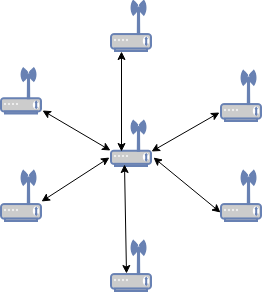
\includegraphics[scale=0.9]{ex_radio.png} 
\caption{Exemple de communication radio}
\end{figure}


\newpage
\section{Exemples de simulations graphiques}
Afin de simplifié, les messages contiennent le nom du message et possedent un code couleur propre et unique. Une \textit{LoRa} Gateway possède une couleur propre à son groupe ( elle même et les Isolated nodes associés), les INs ont aussi cette couleur.
\subsection{Simulation sur une chaine}
\begin{figure}[!ht]
\centering
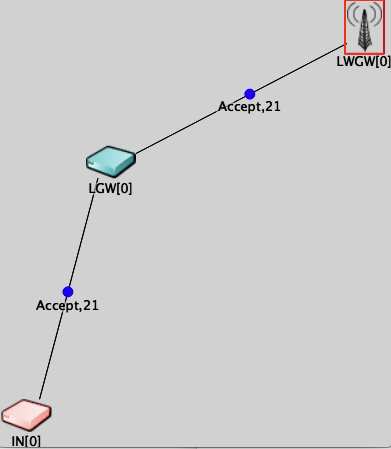
\includegraphics[scale=0.6]{chaine.png} 
\caption{Exemple de chaine}
\end{figure}
Ceci est une image sortie de la simulation graphique, la première réalisé, un exemple typique de chaine avec seulement un élement de chaque composant. C'est le premier exemple de test réalisé. Ce fut aussi le terrain de devellopement pour affiner le comportement individuel et verifier le fonctionnement correct de chaque composant. Cette simulation ci seras l'exemple typique du première algorithme.
\newpage
\subsection{Simulation avec 3 IN sur une LGW}
\begin{figure}[!ht]
\centering
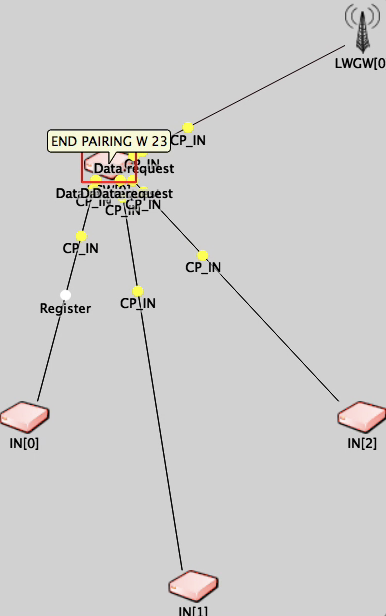
\includegraphics[scale=0.6]{3IN.png} 
\caption{Exemple avec 3 Isolated Nodes}
\end{figure}
Ceci est le deuxième exemple de simulation pour gérer l'enregistrement multiple.Ici nous avons donc toujours une  \textit{LoRaWAN} gateway qui est connecté a une \textit{LoRa} Gateway qui doit gérer trois Isolated Node Cette simulation ci seras l'exemple typique du deuxième algorithme.
\newpage
\subsection{Simulation à plus grande echelle }
\begin{figure}[!ht]
\centering
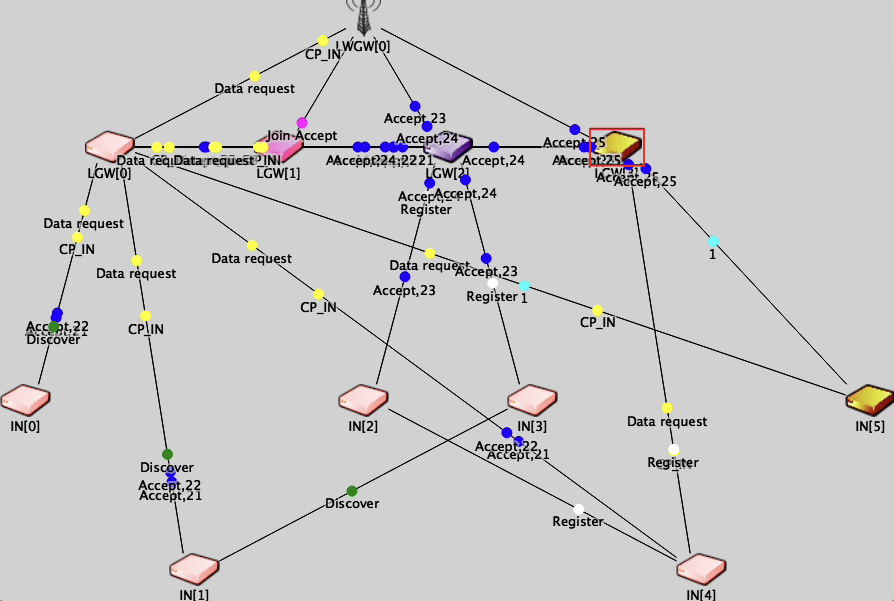
\includegraphics[scale=0.45]{fat.png} 
\caption{Exemple à grande echelle}
\end{figure}
Ceci est le troisème exemple de simulation pour gérer l'enregistrement multiple ainsi que l'unicité d'un enregistrement sur une Gateway \textit{LoRa} d'un device.Ici nous avons donc toujours une  \textit{LoRaWAN} gateway qui est connecté a quatre \textit{LoRa} Gateway qui doit gérer X Isolated Node Cette simulation ci seras l'exemple typique du deuxième algorithme. Mais aussi d'un troisème cas de figure possible. Cette exemple est surtout présent pour montrer et pousser la simulation à être plus proche de la réalité.
L'exemple présenté ci-contre fait aussi transparaitre les exemples ou les communications sont difficiles. Un noeud peut pendant un certain temps ne faire que envoyer des messages \textbf{Discover} très longtemps. Pour plusieurs raisons, notamment celle-ci : 
\begin{itemize}
\item Problème de latence sur le reseaux de communication. 
\item Problème de bruit radio (Plusieurs emissions sont réalisé en même temps de la part de plusieurs device, que ce soit sur le device de recepetion ou d'émission provocant la corrupition des messages)
\item Problème de phase réception, en effet des slots sont prévue ainsi que deux fenêtre de réception dans la specification \textit{LoRa}. Il se peut que deux device pas encore synchroniser est du mal à l'être .
\end{itemize}

\subsection{Générations des graphes}
Un ensemble de 100 graphes contenant 1000 noeuds on été simulé en respectant cette configuration. 
\begin{itemize}
\item  Variation du nombre de nœuds isolés par passerelle entre 1 et 4.
\item  Variation du nombre de passerelle maximum par puits entre 1 et 4.
\item  Variation du nombre de données à récupérer par jour entre 1 et 24 messages.
\item  Variation sur la méthode de réassemblage des données collectées par les nœuds isolés (ie, envoyé au puits à chaque réception (méthode NA) ou réassemblé après fusion de tous les messages (méthode A))
\item  Variation de la vitesse de chaque lien entre deux nœuds.
\end{itemize}
Ce qui nous fait un total de 12800 graphes à créer. Pour réaliser cette création, nous avons écrit un algorithme basé sur la probabilité d'existence d'un lien entre deux nœuds. C'est-à-dire qu'au début nous créons le premier puits(LWGW). À celui-là regarde son degré (lequel est zéro au début) de la passerelle accrochée à lui. On tire une probabilité et si elle est supérieure à celle établie en entrée de l'algorithme on ajoute une passerelle(LGW) et le lien entre le puits et celui-ci. Nous faisons de même avec les nœuds isolés.
Pour résumer, nous avions:
cent graphiques avec un maximum d'un nœud isolé par passerelle et un maximum d'une passerelle par puits. Cette configuration sera abrégée 1 (IN) -1 (GW) $ \ rightarrow $ 1-1.

Nous avons donc utilisé l'outil Omnet ++ pour simuler tous ces graphes et chaque cas. Dans ceux-ci nous avons noté pour le noeud isolé le nombre de messages envoyés ainsi que la batterie restante à la fin de la simulation.
Pour la batterie, nous avons supposé qu'il avait 6600 mAh ou 23760000 mAs. L'énergie électrique consommée provient de la documentation LoPy, section WiFi. Nos calculs de prévision sont réalisés comme suit:

L'appareil est considéré pour envoyer X msg (\#msg) par jour (sur 24 heures). Le courant d'une émission est Ce = 107,3 ​​mA. Chaque émission dure Te = 2s.
Le courant en réception est Cr = 37mA. L'heure à la réception est Tr
Le courant de veille est Cv = 0,531 mA. L'appareil est inactif pour Tv = (24 * 3600- \#msg * Te-Tr * Cr)
Le courant consommé sur une journée est donc:
CDay (mA.s) = (\#msg * Ceci * Te + Cr * Tr + Cv * Tv)
\subsection{Résultats}
Voici donc un graphique montrant la différence entre le mode d'agrégation et de non-agrégation au niveau du message.
\begin{figure}[htbp]
\centerline{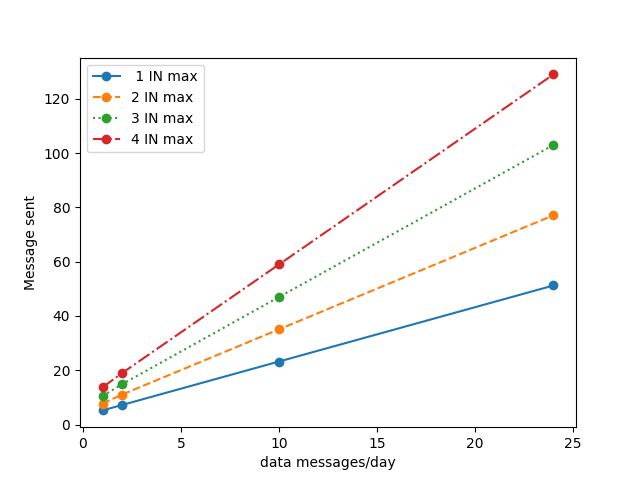
\includegraphics[scale = 0.5]{graphics_resultats/A/A.png}}
\caption{Mode: Agrégation (Concentrateur)}
\label{A}
\end{figure}
On peut remarquer que dans les figures suivantes un aspect linéaire ressort nettement sur la variation du nombre de messages de la part d'une passerelle quel que soit le mode (avec agrégation ou sans agrégation).
\begin{figure}[htbp]
\centerline {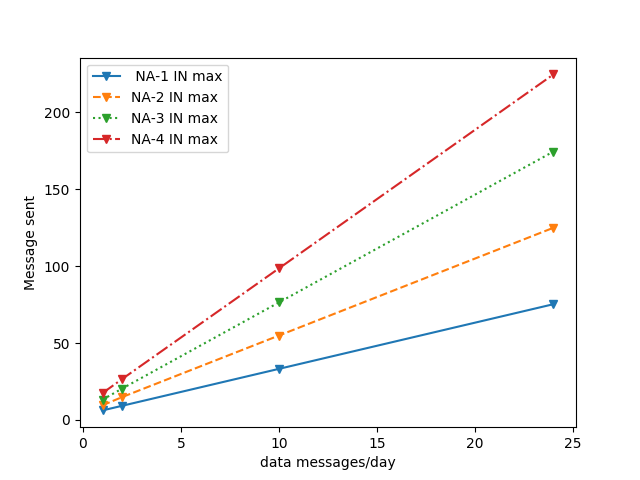
\includegraphics[scale = 0.5]{graphics_resultats/A/NA.png}}
\caption{Mode: Sans d'agrégation (PROXY)}
\label{A}
\end{figure}
Ce que nous pouvons également remarquer est le nombre qui, comme prévu, est plus grand et croît beaucoup plus vite sans le mode d'agrégation (Fig. 4, 5, 6).
Ce qui peut donc être considéré comme suffisamment significatif. En effet, l'ajout des données de la passerelle à celles des noeuds isolés fait que le nombre de messages en mode cluster est le même que si les IN étaient des GW et donc des noeuds connectés.
\begin{figure}[htbp]
\centerline{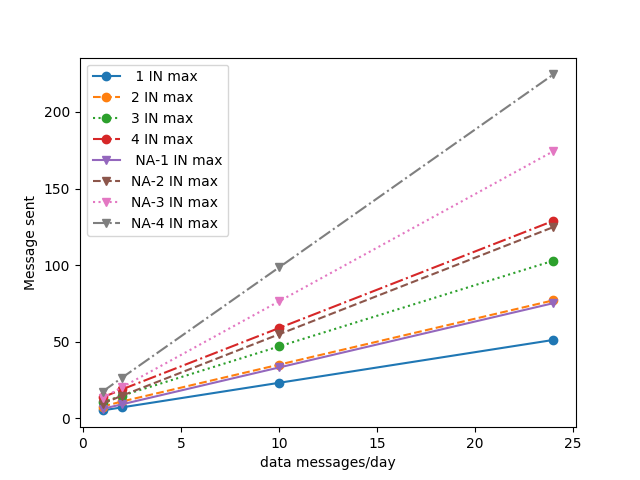
\includegraphics[scale = 0.5]{graphics_resultats/A/AvsNA.png}}
\caption{Mode: Concentrateur vs Proxy}
\label{A}
\end{figure}

L'objectif était de vérifier si l'idée intuitive est correcte: l'architecture avec relais intermédiaire et agrégation renvoie, en nombre de messages et donc de durée de vie du réseau, au modèle sans relais, le modèle ou chaque client parle en direct avec des antennes toujours UP.

Les figures 7 à 10 sont plus complexes. En effet ces graphes représentent par leurs couleurs le nombre de Gateway maximum lié à un puits. Chaque point est un rappel de simulation décrit par le degré maximum de passerelles et de nœuds isolés ainsi que le nombre de messages demandés par le puits par jour. Ici, ces quatre figures sont en mode d'agrégation.

D'abord sur chaque graphique, chaque point est une moyenne du nombre de messages envoyés ou de l'état de la batterie le cas échéant, par un nœud isolé, ou par une passerelle si nécessaire. Pour chaque graphe, le bloc de 4 couleurs est donc l'ensemble des graphes de degré 1 IN. il faut comprendre que les simulations de 0 à 399 sont celles appelées "1-1, 1-2, 1-3, 1-4". de 400 à 799 "2-1, 2-2, 2-3, 2-4" etc.
Nous avons réalisé ces simulations avec comme précédemment dit un nombre de message demandé par les différents puits. En effet nous avons choisi: 1, 2, 10, 24 messages par jour.
\begin{figure}[!ht]
\centerline {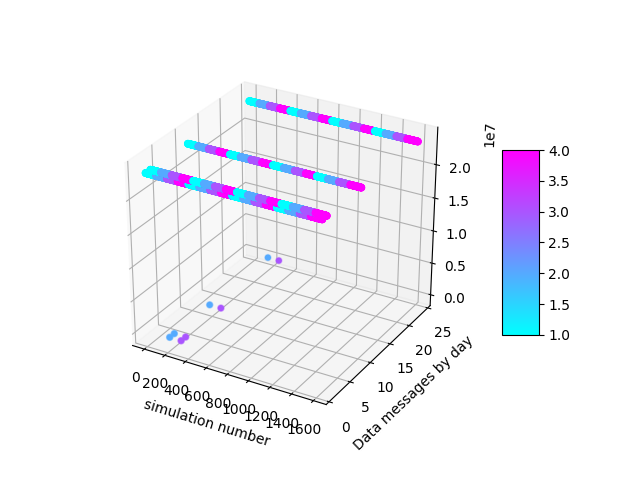
\includegraphics[scale=0.5]{graphics_resultats/bat/Sim_MSG_SEND_data_bat_gw_degree_gw.png}}
\caption {Etat de la batterie sur un jour / message de données requis / jour pour une passerelle}
\label{A}
\end{figure}

\begin{figure}[!ht]
\centerline{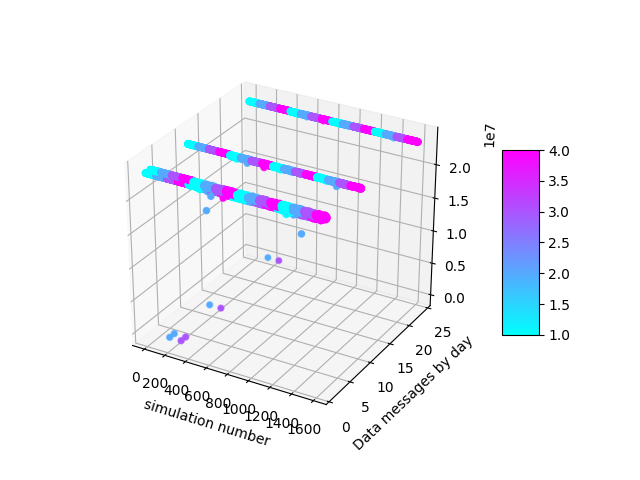
\includegraphics[scale = 0.5]{graphics_resultats/bat/Sim_MSG_SEND_data_bat_in_degree_GW.png}}
\caption{Etat de la batterie sur un jour / message de données requis / jour pour un IN}
\label{A}
\end{figure}


\begin{figure}[!ht]
\centerline {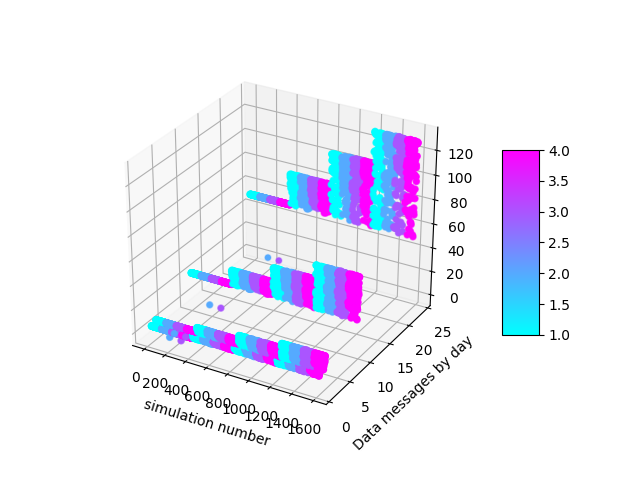
\includegraphics[scale = 0.5]{graphics_resultats/msg/Sim-MSG_GW-MSG_SEND-degree_GW.png}}
\caption {Nombre de messages sur un jour / message de données}
\end{figure}